\chapter{Replikasi DNA dan Mitosis}\label{ch:b1:replication-mitosis}

Kira-kira tiap delapan jam, sebuah \omterm{def:b1:cell-unit-of-life:cell}{sel} pelapis usus menyalin enam
miliar \omterm{thm:b1:nucleic-acids:helix}{pasangan basa} dengan sekitar satu kekeliruan tiap semiliar, lalu
memilah kedua salinannya ke dalam dua \omterm{def:b1:cell-unit-of-life:cell}{sel} anak sehingga masing-masing
memperoleh tepat empat puluh enam \omterm{def:b1:genomes:genome}{kromosom} --- bukan empat puluh lima,
bukan empat puluh tujuh. Penyalinannya dikerjakan sebuah mesin yang
membaca satu untai lalu membangun pasangannya pada lima puluh huruf tiap
sekon dari puluhan ribu titik awal sekaligus; pemilahannya dikerjakan
sebuah \omterm{def:b1:replication-mitosis:mitosis}{gelendong} \omterm{def:b1:eukaryotic-cell:cytoskeleton}{mikrotubul} yang menarik kedua salinan tiap \omterm{def:b1:genomes:genome}{kromosomnya}
terpisah dengan ketepatan satu kekeliruan tiap seratus ribu pembelahan.
Bab ini memerikan \omterm{def:b1:replication-mitosis:fork}{garpu replikasi} beserta \omterm{def:b1:enzymes:enzyme}{enzimnya}, masalah ujungnya,
\omterm{def:b1:replication-mitosis:cycle}{daur sel} yang mengatur waktu replikasi serta pembelahannya, dan \omterm{def:b1:replication-mitosis:mitosis}{mitosis},
yaitu pembelahannya sendiri.

\section{Replikasi semikonservatif}

\begin{proposition}[Tiap untai menjadi cetakan]\label{prop:b1:replication-mitosis:semiconservative}
\index{replikasi semikonservatif}
\omterm{def:b1:nucleic-acids:chain}{DNA} direplikasi secara \emph{semikonservatif}: kedua untai heliksnya
terpisah, dan masing-masing berperan sebagai cetakan tempat sebuah untai
pelengkap yang baru dibangun, sehingga tiap molekul anaknya adalah satu
untai lama yang berpasangan dengan satu untai baru.
\end{proposition}
\begin{proof}[Bukti eksperimental]
Meselson dan Stahl (1958; diingat kembali dari jilid Sekolah Menengah)
menumbuhkan \emph{E. coli} pada nitrogen berat, memindahkannya ke
nitrogen ringan, lalu memisahkan \omterm{def:b1:nucleic-acids:chain}{DNA-nya} menurut massa jenis: sesudah
satu generasi seluruh \omterm{def:b1:nucleic-acids:chain}{DNA-nya} bermassa jenis pertengahan, sesudah dua
generasi separuhnya pertengahan dan separuhnya ringan --- tepat ramalan
satu untai lama dan satu untai baru tiap molekulnya, dan bukan ramalan
skema mana pun yang lain. Cairns (1963) menandai \omterm{def:b1:genomes:genome}{kromosom} bakteri yang
sedang bereplikasi dengan tritium lalu memotretnya lewat autoradiografi:
lingkaran dengan sebuah ``gelembung'' replikasi yang kedua garpunya
bergerak berlawanan arah dari satu titik awal. Kornberg (1956) memurnikan
sebuah \omterm{def:b1:enzymes:enzyme}{enzim} yang mensintesis \omterm{def:b1:nucleic-acids:chain}{DNA} dalam tabung uji dari keempat
nukleosida trifosfatnya dan sebuah cetakan, menurut urutan cetakannya.
\end{proof}

\begin{definition}[Garpu replikasi dan enzimnya]\label{def:b1:replication-mitosis:fork}
\index{garpu replikasi}\index{DNA polimerase}\index{fragmen Okazaki}
Replikasi mulai pada sebuah \emph{titik awal} --- satu pada \omterm{def:b1:genomes:genome}{kromosom}
bakteri, puluhan ribu pada sebuah \omterm{def:b1:genomes:genome}{genom} eukariot --- tempat heliksnya
dibuka dan dua \emph{garpu replikasi} bergerak menjauh ke arah yang
berlawanan. Pada tiap garpunya: sebuah \emph{helikase} mengurai
heliksnya (satu \omterm{def:b1:water-small-molecules:atp}{ATP} tiap \omterm{thm:b1:nucleic-acids:helix}{pasangan basa}), \emph{\omterm{def:b1:proteins:peptide}{protein} pengikat untai
tunggal} menjaga untai yang terpisah itu tetap terpisah, dan sebuah
\emph{topoisomerase} di depan garpunya melepaskan pilinan yang ditimbun
penguraiannya. \emph{\omterm{def:b1:nucleic-acids:chain}{DNA} polimerase} hanya menambahkan \omterm{def:b1:nucleic-acids:nucleotide}{nukleotida} pada
hidroksil $3'$ sebuah rantai yang sudah ada, sehingga tiap untai baru
tumbuh $5' \to 3'$ dan tak satu pun dapat memulai dari ketiadaan: sebuah
\emph{primase} lebih dahulu menaruh sebuah \emph{primer} \omterm{def:b1:nucleic-acids:chain}{RNA} pendek yang
lalu diperpanjang polimerasenya. Pada cetakan yang dibaca $3' \to 5'$
untai barunya tumbuh sinambung ke arah garpunya: \emph{untai pemimpin}.
Pada cetakan yang lain untai barunya harus tumbuh menjauhi garpunya,
dalam keping berisi \qtyrange{1000}{2000}{} \omterm{def:b1:nucleic-acids:nucleotide}{nukleotida} pada bakteri dan
\qtyrange{100}{200}{} pada eukariot, yaitu \emph{fragmen Okazaki}, yang
masing-masing berprimer sendiri: \emph{untai tertinggal}. Sebuah
polimerase kedua mengganti primernya dengan \omterm{def:b1:nucleic-acids:chain}{DNA} dan sebuah \emph{ligase}
menyegel fragmennya menjadi satu untai.
\end{definition}

\begin{omfigure}
\begin{tikzpicture}[font=\footnotesize, >=Stealth, line cap=round]
  % parental duplex on the right, opening leftward
  \draw[very thick, omDef] (12.4,1.0) -- (7.6,1.0);
  \draw[very thick, omDef!50] (12.4,-1.0) -- (7.6,-1.0);
  \foreach \x in {8.0,8.6,...,12.2} { \draw[thick, gray!60] (\x,1.0) -- (\x,-1.0); }
  \node[anchor=south] at (10.0,1.15) {dupleks induk};
  % helicase at the fork
  \node[circle, draw, thick, fill=omProp!40, minimum size=9mm, font=\scriptsize] (hel) at (7.3,0) {helikase};
  \draw[->, very thick, omProp!80!black] (6.4,-1.9) -- (5.2,-1.9) node[left, font=\scriptsize] {garpu bergerak};
  % separated template strands going left
  \draw[very thick, omDef] (7.0,0.55) .. controls (5.5,1.5) .. (0.4,2.2);
  \draw[very thick, omDef!50] (7.0,-0.55) .. controls (5.5,-1.5) .. (0.4,-2.2);
  \node[anchor=east, omDef] at (0.3,2.2) {$3'$};
  \node[anchor=east, omDef!70!black] at (0.3,-2.2) {$5'$};
  % leading strand: continuous new strand along upper template
  \draw[very thick, omThm] (1.0,1.85) .. controls (4.5,1.35) .. (6.2,0.75);
  \node[draw, thick, fill=omThm!25, rounded corners=3pt, inner sep=2pt, font=\scriptsize] at (6.0,0.95) {pol};
  \node[anchor=south west, omThm, align=left] at (1.0,2.35) {untai pemimpin: sinambung, $5' \to 3'$ ke arah garpunya};
  \node[anchor=east, omThm] at (0.95,1.85) {$5'$};
  % lagging strand: Okazaki fragments along lower template, each with a primer
  \foreach \x/\y in {1.2/-1.95, 3.3/-1.55, 5.3/-1.05} {
    \fill[omExo!80!black] (\x,\y) circle (0.08);
    \draw[very thick, omThm] (\x,\y) .. controls (\x+0.8,\y+0.15) .. (\x+1.5,\y+0.25);
  }
  \node[draw, thick, fill=omThm!25, rounded corners=3pt, inner sep=2pt, font=\scriptsize] at (6.7,-1.0) {pol};
  \node[anchor=north west, align=left] at (1.0,-2.5) {untai tertinggal: fragmen Okazaki, masing-masing dimulai sebuah primer RNA (\textcolor{omExo!80!black}{titik}),\\ yang tumbuh $5' \to 3'$ menjauhi garpunya; primernya diganti, fragmennya disambung ligase};
  \node[font=\scriptsize, anchor=south] at (3.3,-1.35) {$5'$};
\end{tikzpicture}

{\small Sebuah \omterm{def:b1:replication-mitosis:fork}{garpu replikasi}. Helikasenya membuka dupleks induknya;
untai pemimpinnya disalin sinambung ke arah garpunya, untai
tertinggalnya mundur dalam \omterm{def:b1:replication-mitosis:fork}{fragmen Okazaki}, sebab polimerase hanya
membangun pada arah $5' \to 3'$.}
\end{omfigure}

\begin{proposition}[Kesetiaan]\label{prop:b1:replication-mitosis:fidelity}
\index{pengoreksian}
Pemasangan basa sendirian akan memberikan sekitar satu kekeliruan tiap
$10^5$; polimerasenya \emph{mengoreksi} --- sebuah keaktifan
eksonuklease $3' \to 5'$ menyingkirkan \omterm{def:b1:nucleic-acids:nucleotide}{nukleotida} yang salah pasang
sebelum yang berikutnya ditambahkan --- sehingga kekeliruannya menjadi
satu tiap $10^7$; dan sesudah garpunya lewat, sebuah sistem
\emph{perbaikan salah pasang} menemukan salah pasang yang tersisa,
mengenali untai barunya, lalu memperbaikinya: satu kekeliruan tiap
$10^9$ sampai $10^{10}$ \omterm{thm:b1:nucleic-acids:helix}{pasangan basa} tiap replikasi. Sebuah \omterm{def:b1:cell-unit-of-life:cell}{sel} manusia
yang menyalin $\num{6.4e9}$ pasangan membuat segelintir mutasi tiap kali
ia membelah; sebuah bakteri, satu tiap seribu pembelahan.
\end{proposition}

\begin{example}[Kecepatan dan titik awalnya]\label{ex:b1:replication-mitosis:speed}
Sebuah garpu bakteri bergerak \qty{1000}{} \omterm{thm:b1:nucleic-acids:helix}{pasangan basa} tiap sekon: dua
garpu menyalin \qty{4.6}{Mb} \emph{E. coli} dalam \qty{40}{min}, dan
dalam medium kaya, tempat \omterm{def:b1:cell-unit-of-life:cell}{selnya} membelah tiap dua puluh menit, sebuah
putaran baru mulai sebelum yang terakhir selesai. Sebuah garpu eukariot,
yang diperlambat kromatinnya, bergerak \qty{50}{} tiap sekon: menyalin
sebuah \omterm{def:b1:genomes:genome}{kromosom} manusia \qty{250}{Mb} dari satu titik awal akan memakan
waktu sebulan, sehingga \omterm{def:b1:genomes:genome}{genomnya} disalin dari sekitar \num{40000} titik
awal dalam delapan jam, dalam urutan yang tertentu bagi tiap jenis
\omterm{def:b1:cell-unit-of-life:cell}{selnya}.
\end{example}

\section{Ujungnya}

\begin{proposition}[Masalah replikasi ujung dan telomerase]\label{prop:b1:replication-mitosis:telomerase}
\index{telomerase}
Pada sebuah \omterm{def:b1:genomes:genome}{kromosom} lurus untai tertinggalnya tak dapat dilengkapi
sampai ujung sekali: ketika primer terakhirnya disingkirkan tak ada
hidroksil $3'$ di hulunya untuk mengisi celahnya, dan tiap replikasinya
akan memendekkan \omterm{def:b1:genomes:genome}{kromosomnya} sebesar \qtyrange{50}{100}{} \omterm{def:b1:nucleic-acids:nucleotide}{nukleotida}.
Eukariot mengakhiri \omterm{def:b1:genomes:genome}{kromosomnya} dengan \emph{\omterm{def:b1:genomes:karyotype}{telomer}}, yaitu ribuan
salinan sebuah ulangan pendek (TTAGGG pada vertebrata) yang tidak
membawa \omterm{def:b1:genomes:gene}{gen}, dan \omterm{def:b1:cell-unit-of-life:cell}{sel} kelamin serta \omterm{def:b1:cell-unit-of-life:cell}{sel} punca membawa
\emph{telomerase}, sebuah \omterm{def:b1:enzymes:enzyme}{enzim} dengan cetakan \omterm{def:b1:nucleic-acids:chain}{RNA-nya} sendiri yang
menambahkan ulangan pada ujung $3'$-nya, sehingga memulihkan apa yang
hilang oleh replikasinya. Sebagian besar \omterm{def:b1:cell-unit-of-life:cell}{sel} tubuh tidak memilikinya:
\omterm{def:b1:genomes:karyotype}{telomernya} memendek pada tiap pembelahan, dan sesudah sekitar lima
puluh pembelahan dalam \omterm{def:b1:cell-unit-of-life:culture}{biakan sel} itu berhenti membelah. Bakteri, yang
\omterm{def:b1:genomes:genome}{kromosomnya} melingkar, tidak memiliki ujung.
\end{proposition}

\begin{omfigure}
\begin{tikzpicture}[font=\footnotesize, >=Stealth, line cap=round]
  % top: the problem
  \draw[very thick, omDef] (0,1.2) -- (8,1.2) node[right] {$3'$ (cetakan)};
  \draw[very thick, omThm] (0,0.8) -- (6.3,0.8);
  \fill[omExo!80!black] (6.3,0.8) circle (0.08); \draw[very thick, omExo!80!black] (6.3,0.8) -- (7.0,0.8);
  \node[anchor=east, omThm] at (-0.1,0.8) {untai tertinggal baru $5'$};
  \node[anchor=north, font=\scriptsize, omExo!80!black] at (6.65,0.72) {primer terakhir};
  \draw[thick, gray] (7.0,0.55) -- (8.0,0.55);
  \node[anchor=north, font=\scriptsize, align=center, gray] at (7.5,0.45) {celah: tak ada yang dapat diperpanjang\\ begitu primernya disingkirkan};
  % bottom: telomerase
  \draw[very thick, omDef] (0,-1.6) -- (8,-1.6);
  \draw[very thick, omDef, dashed] (8,-1.6) -- (10.2,-1.6) node[right] {$3'$ diperpanjang};
  \node[draw, thick, fill=omProp!30, rounded corners=4pt, inner sep=3pt, align=center, font=\scriptsize] at (9.1,-0.95) {telomerase\\ (cetakan RNA di dalamnya)};
  \draw[very thick, omThm] (0,-2.0) -- (6.3,-2.0);
  \draw[very thick, omThm, dashed] (6.3,-2.0) -- (8.6,-2.0);
  \node[anchor=east, align=right, font=\scriptsize] at (-0.1,-1.8) {ulangan telomer\\ TTAGGG\ldots};
  \node[anchor=north, align=center, gray] at (5,-2.3) {telomerase memanjangkan ujung $3'$ cetakannya dengan ulangan; sebuah primer baru pada\\ perpanjangannya membuat untai tertinggalnya dapat dilengkapi sampai panjang semula};
\end{tikzpicture}

{\small Masalah replikasi ujungnya (atas) dan pemecahannya (bawah).
Untai tertinggalnya tertinggal pendek pada ujung \omterm{def:b1:genomes:genome}{kromosomnya};
telomerase menambahkan ulangan pada ujung $3'$ cetakannya sehingga
kehilangannya jatuh pada urutan yang tidak membawa \omterm{def:b1:genomes:gene}{gen}.}
\end{omfigure}

\section{Daur sel}

\begin{definition}[Daur sel]\label{def:b1:replication-mitosis:cycle}
\index{daur sel}\index{interfase}
\emph{Daur \omterm{def:b1:cell-unit-of-life:cell}{sel}} sebuah \omterm{def:b1:cell-unit-of-life:prokeuk}{sel eukariot} memiliki empat fase.
\emph{G$_1$} (jeda 1): \omterm{def:b1:cell-unit-of-life:cell}{selnya} tumbuh dan membuat \omterm{def:b1:enzymes:enzyme}{enzim} replikasinya;
\emph{S} (sintesis): ia mereplikasi \omterm{def:b1:nucleic-acids:chain}{DNA-nya}, sehingga tiap \omterm{def:b1:genomes:genome}{kromosomnya}
menjadi dua \emph{\omterm{def:b1:replication-mitosis:mitosis}{kromatid} saudari} yang serupa dan bergabung pada
\omterm{def:b1:genomes:karyotype}{sentromernya}; \emph{G$_2$}: ia tumbuh lebih jauh dan memeriksa
salinannya; \emph{M}: \emph{\omterm{def:b1:replication-mitosis:mitosis}{mitosis}}, yaitu pembelahan \omterm{def:b1:cell-unit-of-life:prokeuk}{intinya}, yang
diikuti \emph{sitokinesis}, yaitu pembelahan \omterm{def:b1:cell-unit-of-life:cell}{sitoplasmanya}. G$_1$, S dan
G$_2$ bersama-sama adalah \emph{interfase}, ketika \omterm{def:b1:genomes:genome}{kromosomnya}
terentang dan aktif; sebuah \omterm{def:b1:cell-unit-of-life:cell}{sel} yang berhenti membelah meninggalkan
daurnya dari G$_1$ ke sebuah keadaan istirahat, G$_0$. Sebuah \omterm{def:b1:cell-unit-of-life:cell}{sel}
manusia yang membelah memakan waktu sekitar
\qty{24}{h}: G$_1$ \qty{10}{h}, S \qty{8}{h}, G$_2$ \qty{4}{h}, M
\qty{1}{h}; sebuah khamir, \qty{90}{min}; sebuah embrio katak awal, tiga
puluh menit tanpa jeda sama sekali.
\end{definition}

\begin{omfigure}
\begin{tikzpicture}
\begin{axis}[
  width=0.9\linewidth, height=5.6cm,
  axis x line=bottom, axis y line=left,
  xmin=0, xmax=26, ymin=0, ymax=2.6,
  xlabel={waktu (h)}, ylabel={DNA tiap inti},
  xlabel style={font=\small, at={(axis description cs:0.5,-0.14)}, anchor=north},
  ylabel style={font=\small},
  tick label style={font=\small}, xtick={0,10,18,22,23,24}, xticklabels={0,10,18,22,23,24},
  ytick={1,2}, yticklabels={$q$,$2q$},
  clip=false,
]
\addplot[very thick, omDef] coordinates {(0,1) (10,1) (18,2) (23,2) (23.6,2) (23.6,1) (24,1) (26,1)};
\fill[omDef!12] (axis cs:0,2.25) rectangle (axis cs:10,2.55); \node[font=\scriptsize] at (axis cs:5,2.4) {G$_1$: pertumbuhan};
\fill[omThm!15] (axis cs:10,2.25) rectangle (axis cs:18,2.55); \node[font=\scriptsize] at (axis cs:14,2.4) {S: replikasi};
\fill[omDef!12] (axis cs:18,2.25) rectangle (axis cs:22,2.55); \node[font=\scriptsize] at (axis cs:20,2.4) {G$_2$};
\fill[omExo!25] (axis cs:22,2.25) rectangle (axis cs:24,2.55); \node[font=\scriptsize] at (axis cs:23,2.4) {M};
\node[font=\scriptsize, anchor=west, align=left] at (axis cs:24.1,1.5) {dua sel,\\ $q$ masing-masing};
\end{axis}
\end{tikzpicture}

{\small Kandungan \omterm{def:b1:nucleic-acids:chain}{DNA} sebuah \omterm{def:b1:cell-unit-of-life:prokeuk}{inti} sepanjang satu \omterm{def:b1:replication-mitosis:cycle}{daur sel} \qty{24}{h}.
Kandungan itu berlipat dua selama fase S, dari $q$ (2n \omterm{def:b1:genomes:genome}{kromosom}
berkromatid satu) menjadi $2q$ (2n \omterm{def:b1:genomes:genome}{kromosom} berkromatid dua), lalu
kembali ke $q$ pada tiap \omterm{def:b1:cell-unit-of-life:cell}{sel} anaknya pada akhir \omterm{def:b1:replication-mitosis:mitosis}{mitosisnya}; banyaknya
\omterm{def:b1:genomes:genome}{kromosom} tak pernah berubah.}
\end{omfigure}

\begin{proposition}[Titik pemeriksaan]\label{prop:b1:replication-mitosis:checkpoints}
\index{titik pemeriksaan}
Daurnya digerakkan maju sebuah keluarga \omterm{def:b1:proteins:peptide}{protein} kinase, yang
diaktifkan bergiliran oleh \omterm{def:b1:proteins:peptide}{protein} yang disebut \emph{siklin} yang
arasnya naik turun sepanjang daurnya, dan ia ditahan pada \emph{\omterm{prop:b1:replication-mitosis:checkpoints}{titik
pemeriksaan}} sampai syaratnya terpenuhi: pada akhir G$_1$, \omterm{def:b1:cell-unit-of-life:cell}{selnya}
berkomitmen untuk mereplikasi hanya bila ia cukup besar, cukup makanan
dan diberi isyarat untuk membelah, serta bila \omterm{def:b1:nucleic-acids:chain}{DNA-nya} tidak rusak; pada
akhir G$_2$, ia masuk ke \omterm{def:b1:replication-mitosis:mitosis}{mitosis} hanya ketika replikasinya lengkap;
dalam \omterm{def:b1:replication-mitosis:mitosis}{mitosis}, \omterm{def:b1:replication-mitosis:mitosis}{kromatidnya} terpisah hanya ketika tiap \omterm{def:b1:genomes:genome}{kromosomnya}
terpaut pada \omterm{def:b1:replication-mitosis:mitosis}{gelendongnya} dari kedua sisinya. Kerusakan menghentikan
daurnya dan, bila tak dapat diperbaiki, memicu kematian \omterm{def:b1:cell-unit-of-life:cell}{selnya}. Mesin
molekul kendali ini menjadi bagian jilid Tahun ke-3; kegagalannya
adalah kanker.
\end{proposition}

\section{Mitosis}

\begin{definition}[Mitosis]\label{def:b1:replication-mitosis:mitosis}
\index{mitosis}\index{gelendong}\index{kromatid}
\emph{Mitosis} membagikan \omterm{def:b1:genomes:genome}{kromosom} yang telah direplikasi sehingga tiap
\omterm{def:b1:cell-unit-of-life:prokeuk}{inti} anaknya menerima satu kromatid tiap \omterm{def:b1:genomes:genome}{kromosomnya} --- dengan cacah
dan \omterm{def:b1:genomes:gene}{gen} yang sama dengan induknya. Tahapnya:
\begin{itemize}
  \item \emph{profase}: \omterm{def:b1:genomes:genome}{kromosomnya} memadat menjadi \omterm{def:b1:flowering-plant-organization:organs}{batang} yang tampak,
        masing-masing berisi dua kromatid saudari yang dipegang bersama
        sepanjang tubuhnya oleh \omterm{def:b1:proteins:peptide}{protein} kohesin; kedua
        \emph{\omterm{def:b1:eukaryotic-cell:cytoskeleton}{sentrosom}}nya bergerak menjauh dan \emph{gelendong
        mitosis} dari \omterm{def:b1:eukaryotic-cell:cytoskeleton}{mikrotubul} tumbuh di antaranya;
  \item \emph{prometafase}: \omterm{def:b1:eukaryotic-cell:nucleus}{selubung intinya} rusak; \omterm{def:b1:eukaryotic-cell:cytoskeleton}{mikrotubul}
        gelendongnya melekat pada \emph{kinetokor} tiap kromatidnya,
        yaitu sebuah struktur \omterm{def:b1:proteins:peptide}{protein} pada \omterm{def:b1:genomes:karyotype}{sentromernya}, dari kutub yang
        berlawanan;
  \item \emph{metafase}: \omterm{def:b1:genomes:genome}{kromosomnya} berjajar pada khatulistiwa
        gelendongnya, masing-masing tertarik dari kedua kutubnya;
  \item \emph{anafase}: kohesinnya dipotong, kromatid saudarinya
        terpisah lalu ditarik ke kutub yang berlawanan seiring
        memendeknya \omterm{def:b1:eukaryotic-cell:cytoskeleton}{mikrotubulnya} (anafase A) dan menjauhnya kutubnya
        (anafase B);
  \item \emph{telofase}: \omterm{def:b1:genomes:genome}{kromosomnya} mengurai, dan sebuah \omterm{def:b1:eukaryotic-cell:nucleus}{selubung inti}
        terbentuk kembali mengelilingi tiap perangkatnya.
\end{itemize}
\emph{Sitokinesis} lalu membelah \omterm{def:b1:cell-unit-of-life:cell}{sitoplasmanya}: pada \omterm{def:b1:cell-unit-of-life:cell}{sel} hewan sebuah
\emph{cincin kerut} dari aktin dan miosin menjepit \omterm{def:b1:cell-unit-of-life:cell}{selnya} menjadi dua;
pada \omterm{def:b1:cell-unit-of-life:cell}{sel} tumbuhan vesikel dari Golgi melebur pada khatulistiwanya
menjadi sebuah \emph{pelat \omterm{def:b1:cell-unit-of-life:cell}{sel}} yang tumbuh ke luar menjadi dinding baru.
\end{definition}

\begin{omfigure}
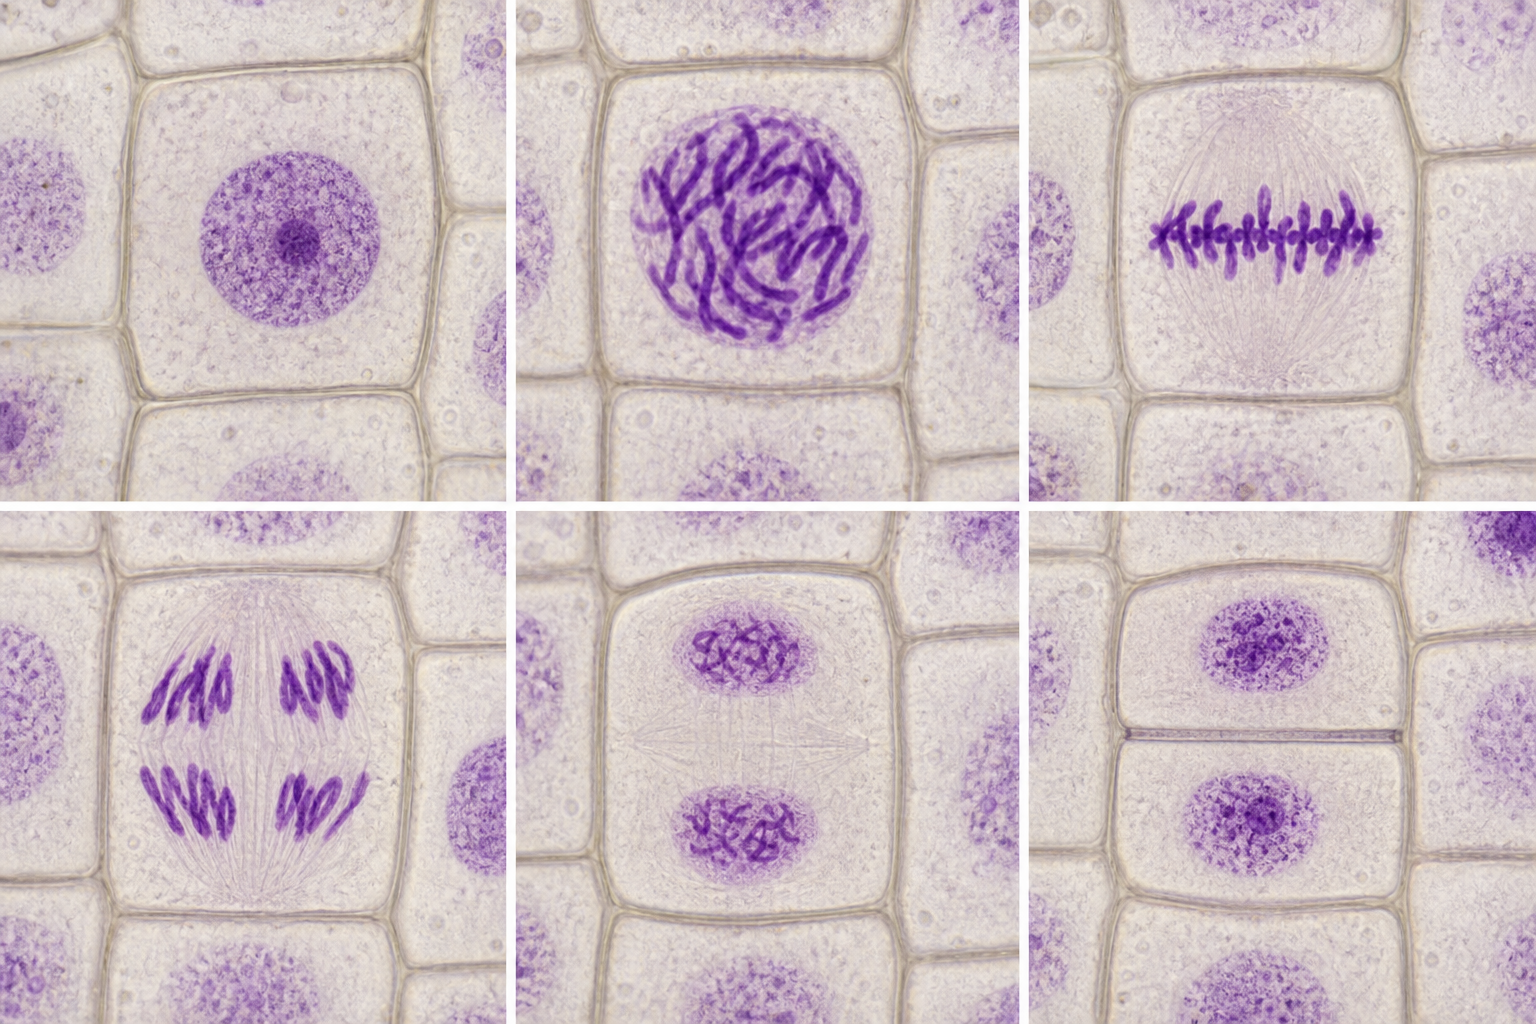
\includegraphics[width=0.9\linewidth]{images/book3/ai/b3-18-mitosis-grid.png}

{\small \omterm{def:b1:cell-unit-of-life:cell}{Sel} ujung \omterm{def:b1:flowering-plant-organization:organs}{akar} bawang dalam \omterm{def:b1:replication-mitosis:cycle}{interfase}, profase, metafase,
anafase, telofase, dan sesudah sitokinesis dengan dinding barunya
melintang di tengahnya. \omterm{def:b1:genomes:genome}{Kromosomnya} hanya tampak selama memadat, dari
profase sampai telofase.}
\end{omfigure}

\begin{omfigure}
\begin{tikzpicture}[font=\footnotesize, >=Stealth, line cap=round]
  \foreach \i/\name in {0/prophase, 1/metaphase, 2/anaphase, 3/telophase} {
    \begin{scope}[xshift=\i*3.3cm]
      \draw[thick, omDef!70!black, fill=omDef!5] (0,0) ellipse (1.4 and 1.1);
      \node[anchor=north] at (0,-1.2) {\name};
    \end{scope}
  }
  % prophase: two centrosomes, condensed chromosomes (X shapes) scattered, envelope
  \begin{scope}
    \draw[thick, gray, dashed] (0,0) circle (0.8);
    \foreach \p/\a in {(-0.3,0.25)/30, (0.35,-0.1)/-40, (0.05,-0.45)/80} { \draw[very thick, omThm] \p ++(\a:0.22) -- ++(\a+180:0.44); \draw[very thick, omThm] \p ++(\a+60:0.22) -- ++(\a+240:0.44); }
    \fill[omProp!80!black] (-1.1,0.6) circle (0.07); \fill[omProp!80!black] (1.1,-0.6) circle (0.07);
    \foreach \a in {-30,0,30} { \draw[omProp!60!black] (-1.1,0.6) -- ++(\a-20:0.45); \draw[omProp!60!black] (1.1,-0.6) -- ++(\a+160:0.45); }
  \end{scope}
  % metaphase: spindle pole to pole, chromosomes on the plate
  \begin{scope}[xshift=3.3cm]
    \fill[omProp!80!black] (-1.25,0) circle (0.07); \fill[omProp!80!black] (1.25,0) circle (0.07);
    \foreach \y in {-0.5,-0.25,0,0.25,0.5} { \draw[omProp!60!black] (-1.25,0) -- (0,\y); \draw[omProp!60!black] (1.25,0) -- (0,\y); }
    \foreach \y in {-0.5,-0.17,0.17,0.5} { \draw[very thick, omThm] (-0.12,\y-0.14) -- (0.12,\y+0.14); \draw[very thick, omThm] (-0.12,\y+0.14) -- (0.12,\y-0.14); }
  \end{scope}
  % anaphase: chromatids moving to poles (V shapes)
  \begin{scope}[xshift=6.6cm]
    \fill[omProp!80!black] (-1.25,0) circle (0.07); \fill[omProp!80!black] (1.25,0) circle (0.07);
    \foreach \y in {-0.45,-0.15,0.15,0.45} { \draw[omProp!60!black] (-1.25,0) -- (-0.55,\y); \draw[omProp!60!black] (1.25,0) -- (0.55,\y); \draw[very thick, omThm] (-0.55,\y) -- (-0.35,\y+0.12) (-0.55,\y) -- (-0.35,\y-0.12); \draw[very thick, omThm] (0.55,\y) -- (0.35,\y+0.12) (0.55,\y) -- (0.35,\y-0.12); }
  \end{scope}
  % telophase: two nuclei reforming, cleavage furrow
  \begin{scope}[xshift=9.9cm]
    \draw[thick, gray, dashed] (-0.7,0) circle (0.45); \draw[thick, gray, dashed] (0.7,0) circle (0.45);
    \foreach \x in {-0.8,-0.6,0.6,0.8} { \draw[thick, omThm] (\x,-0.2) -- (\x,0.2); }
    \draw[very thick, omExo!70!black] (0,1.1) -- (0,0.55); \draw[very thick, omExo!70!black] (0,-1.1) -- (0,-0.55);
    \node[font=\scriptsize, omExo!70!black, anchor=south] at (0,1.15) {lekuk};
  \end{scope}
\end{tikzpicture}

{\small Empat tahap \omterm{def:b1:replication-mitosis:mitosis}{mitosis} pada sebuah \omterm{def:b1:cell-unit-of-life:cell}{sel} hewan. Profase:
\omterm{def:b1:genomes:genome}{kromosomnya} memadat seiring terbentuknya \omterm{def:b1:replication-mitosis:mitosis}{gelendong} dari kedua
\omterm{def:b1:eukaryotic-cell:cytoskeleton}{sentrosomnya}. Metafase: tiap \omterm{def:b1:genomes:genome}{kromosomnya} duduk pada khatulistiwanya,
terpaut dari kedua kutubnya. Anafase: \omterm{def:b1:replication-mitosis:mitosis}{kromatid} saudarinya ditarik
terpisah. Telofase: dua \omterm{def:b1:cell-unit-of-life:prokeuk}{inti} terbentuk kembali dan lekuknya membelah
\omterm{def:b1:cell-unit-of-life:cell}{selnya}.}
\end{omfigure}

\begin{omfigure}
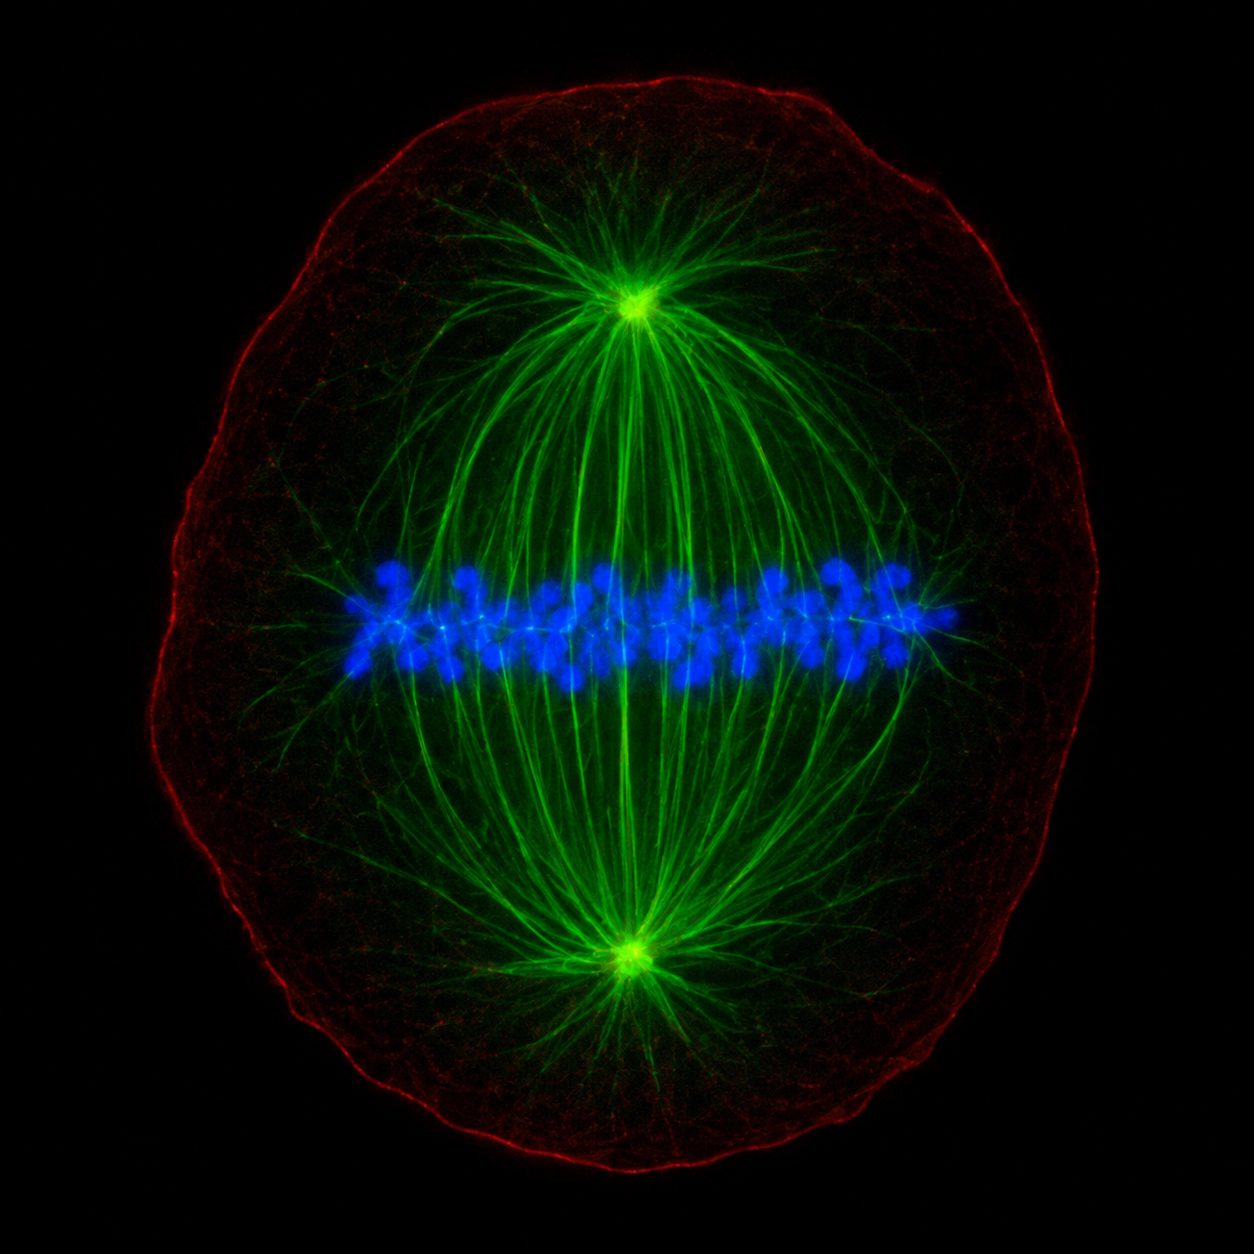
\includegraphics[width=0.4\linewidth]{images/book3/ai/b3-18-mitotic-spindle-fluorescence.png}

{\small Sebuah \omterm{def:b1:cell-unit-of-life:cell}{sel} biakan pada metafase, \omterm{def:b1:eukaryotic-cell:cytoskeleton}{mikrotubulnya} ditandai hijau
dan \omterm{def:b1:genomes:genome}{kromosomnya} biru: \omterm{def:b1:replication-mitosis:mitosis}{gelendongnya} menjangkau \omterm{def:b1:cell-unit-of-life:cell}{selnya} dari kutub ke
kutub dan \omterm{def:b1:genomes:genome}{kromosomnya} membentuk sebuah pelat melintasi khatulistiwanya.}
\end{omfigure}

\begin{proposition}[Apa yang dilestarikan mitosis]\label{prop:b1:replication-mitosis:conserves}
\omterm{def:b1:replication-mitosis:mitosis}{Mitosis} adalah pembelahan yang melestarikan cacah \omterm{def:b1:genomes:genome}{kromosomnya}: sebuah
\omterm{def:b1:cell-unit-of-life:cell}{sel} berkromosom 2n (46 pada manusia) memberikan dua \omterm{def:b1:cell-unit-of-life:cell}{sel} berkromosom 2n.
Kandungan \omterm{def:b1:nucleic-acids:chain}{DNA-nya} bergerak dari $2q$ (sesudah replikasi) ke $q$ pada
tiap \omterm{def:b1:cell-unit-of-life:cell}{sel} anaknya; banyaknya \omterm{def:b1:genomes:genome}{kromosom} tak pernah berubah, sebab sebuah
\omterm{def:b1:genomes:genome}{kromosom} dihitung menurut \omterm{def:b1:genomes:karyotype}{sentromernya}, dan tiap \omterm{def:b1:replication-mitosis:mitosis}{kromatid}, begitu
terpisah, adalah sebuah \omterm{def:b1:genomes:genome}{kromosom}. Karena itu tiap \omterm{def:b1:cell-unit-of-life:cell}{sel} sebuah tubuh
serupa secara genetik dengan \omterm{def:b1:cell-unit-of-life:cell}{sel} telur asalnya, kecuali mutasi yang
dimasukkan penyalinannya. Pembelahan yang membagi dua cacah
\omterm{def:b1:genomes:genome}{kromosomnya}, yaitu meiosis, menjadi bagian jilid Tahun ke-2.
\end{proposition}

\begin{method}[Membaca sebuah percobaan daur sel]\label{met:b1:replication-mitosis:reading}
\begin{enumerate}
  \item Ukurlah \omterm{def:b1:nucleic-acids:chain}{DNA} tiap \omterm{def:b1:cell-unit-of-life:cell}{selnya} (sebuah zat warna yang pendarannya
        sebanding dengan \omterm{def:b1:nucleic-acids:chain}{DNA-nya}, \omterm{def:b1:cell-unit-of-life:cell}{sel} demi \omterm{def:b1:cell-unit-of-life:cell}{sel}): \omterm{def:b1:cell-unit-of-life:cell}{sel} pada $q$ berada
        dalam G$_1$, pada $2q$ dalam G$_2$ atau M, di antaranya dalam S.
        Fraksinya memberikan lamanya: bagian sebuah fase dari daurnya
        adalah bagiannya dari \omterm{def:b1:cell-unit-of-life:cell}{selnya}.
  \item Berikan sebuah denyut \omterm{def:b1:nucleic-acids:nucleotide}{nukleotida} bertanda
        (bromodeoksiuridina): hanya \omterm{def:b1:cell-unit-of-life:cell}{sel} dalam fase S yang menyerapnya;
        fraksi yang bertanda adalah fraksi S-nya, dan mengikuti tandanya
        sampai \omterm{def:b1:replication-mitosis:mitosis}{mitosis} memberikan lama G$_2$-nya.
  \item Hitunglah gambaran \omterm{def:b1:replication-mitosis:mitosis}{mitosis} pada sebuah sayatan yang terwarnai:
        \emph{indeks \omterm{def:b1:replication-mitosis:mitosis}{mitosis}}, yaitu fraksi \omterm{def:b1:cell-unit-of-life:cell}{sel} dalam M, adalah fraksi
        daurnya yang ditempati M --- \qty{4}{\%} bagi daur \qty{24}{h}
        dengan \omterm{def:b1:replication-mitosis:mitosis}{mitosis} satu jam.
  \item Hambatlah satu langkah (sebuah obat yang membongkar \omterm{def:b1:eukaryotic-cell:cytoskeleton}{mikrotubul}
        menahan \omterm{def:b1:cell-unit-of-life:cell}{sel} pada metafase; obat yang menghambat sintesis \omterm{def:b1:nucleic-acids:chain}{DNA}
        menahannya dalam S) lalu hitunglah apa yang menumpuk.
\end{enumerate}
\end{method}

\begin{example}[Perputaran]\label{ex:b1:replication-mitosis:turnover}
\omterm{def:b1:body-plans-tissues:epithelium}{Epitel} usus halus diperbarui tiap empat hari, kulit tiap bulan, \omterm{def:b1:cell-unit-of-life:cell}{sel}
darah merah tiap empat bulan dari sumsumnya, yang menghasilkan dua juta
tiap sekon; sebuah \omterm{def:b1:cell-unit-of-life:cell}{sel} hati membelah kira-kira sekali setahun dan
sebuah \omterm{def:b1:body-plans-tissues:nervous}{neuron} tak pernah. \omterm{def:b1:cell-unit-of-life:cell}{Sel} sebuah tumor telah kehilangan \omterm{prop:b1:replication-mitosis:checkpoints}{titik
pemeriksaannya}: mereka membelah ketika seharusnya tidak, menoleransi
\omterm{def:b1:genomes:genome}{kromosom} yang salah pilah, dan menimbun mutasi yang membuat mereka
membelah lebih cepat lagi. Kemoterapi memanfaatkan perbedaan itu: obat
yang meracuni \omterm{def:b1:replication-mitosis:mitosis}{gelendong} atau polimerasenya membunuh \omterm{def:b1:cell-unit-of-life:cell}{sel} yang paling
banyak membelah.
\end{example}

\section{Latihan}

\begin{exercise}[$\star$]\label{exo:b1:replication-mitosis:1}
Jelaskan mengapa satu untai pada sebuah garpu disalin sinambung dan
untai yang lain dalam keping.
\end{exercise}

\begin{exercise}[$\star$]\label{exo:b1:replication-mitosis:2}
Sebutkan \omterm{def:b1:enzymes:enzyme}{enzim} dan \omterm{def:b1:proteins:peptide}{protein} pada sebuah \omterm{def:b1:replication-mitosis:fork}{garpu replikasi} dan tugas
masing-masing.
\end{exercise}

\begin{exercise}[$\star$]\label{exo:b1:replication-mitosis:3}
Dari gambar kandungan \omterm{def:b1:nucleic-acids:chain}{DNA-nya}, bacalah kandungan \omterm{def:b1:nucleic-acids:chain}{DNA} dalam G$_1$,
G$_2$ dan sesudah \omterm{def:b1:replication-mitosis:mitosis}{mitosis}, serta banyaknya \omterm{def:b1:genomes:genome}{kromosom} pada masing-masing.
\end{exercise}

\begin{exercise}[$\star$]\label{exo:b1:replication-mitosis:4}
Urutkan tahap \omterm{def:b1:replication-mitosis:mitosis}{mitosis} dan berikan peristiwa penentu masing-masing.
\end{exercise}

\begin{exercise}[$\star\star$]\label{exo:b1:replication-mitosis:5}
Hitunglah banyaknya \omterm{def:b1:replication-mitosis:fork}{fragmen Okazaki} yang dibuat saat menyalin \omterm{def:b1:genomes:genome}{genom}
manusia (\num{6.4e9} pasangan, fragmen berisi \qty{150}{}), dan
banyaknya primer, penyingkiran primer serta penyambungan yang
disiratkannya.
\end{exercise}

\begin{exercise}[$\star\star$]\label{exo:b1:replication-mitosis:6}
Hitunglah laju kekeliruan tiap \omterm{def:b1:genomes:genome}{genom} manusia tiap replikasi bagi
sebuah polimerase sendirian ($10^{-5}$), dengan pengoreksian
($10^{-7}$) dan dengan perbaikan salah pasang ($10^{-9}$). Berapa banyak
mutasi yang diberikan masing-masing tiap pembelahan?
\end{exercise}

\begin{exercise}[$\star\star$]\label{exo:b1:replication-mitosis:7}
Sebuah \omterm{def:b1:cell-unit-of-life:cell}{sel} tubuh kehilangan \qty{80}{} \omterm{def:b1:nucleic-acids:nucleotide}{nukleotida} \omterm{def:b1:genomes:karyotype}{telomer} tiap
pembelahan dan mulai dengan \qty{10}{kb}; ia berhenti membelah pada
\qty{5}{kb}. Berapa banyak pembelahan yang dapat dilakukannya? Mengapa
sebuah \omterm{def:b1:cell-unit-of-life:cell}{sel} kanker memerlukan telomerase?
\end{exercise}

\begin{exercise}[$\star\star$]\label{exo:b1:replication-mitosis:8}
Sebuah \omterm{def:b1:body-plans-tissues:tissue}{jaringan} memiliki \qty{5}{\%} \omterm{def:b1:cell-unit-of-life:cell}{selnya} dalam \omterm{def:b1:replication-mitosis:mitosis}{mitosis} dan
\qty{30}{\%} dalam fase S; \omterm{def:b1:replication-mitosis:mitosis}{mitosisnya} berlangsung satu jam. Hitunglah
lama daurnya dan lama fase S-nya.
\end{exercise}

\begin{exercise}[$\star\star$]\label{exo:b1:replication-mitosis:9}
Sebuah \omterm{def:b1:cell-unit-of-life:cell}{sel} memiliki 2n $= 8$. Berikan banyaknya \omterm{def:b1:genomes:genome}{kromosom}, \omterm{def:b1:replication-mitosis:mitosis}{kromatid} dan
kandungan \omterm{def:b1:nucleic-acids:chain}{DNA-nya} (dalam $q$) pada G$_1$, G$_2$, metafase, dan tiap \omterm{def:b1:cell-unit-of-life:cell}{sel}
anak sesudah telofase.
\end{exercise}

\begin{exercise}[$\star\star\star$]\label{exo:b1:replication-mitosis:10}
\emph{E. coli} memerlukan \qty{40}{min} untuk mereplikasi \omterm{def:b1:genomes:genome}{kromosomnya}
tetapi membelah tiap \qty{20}{min} dalam medium kaya. Jelaskan
bagaimana, lalu hitunglah berapa banyak titik awal dan garpu yang dimuat
sebuah \omterm{def:b1:cell-unit-of-life:cell}{sel} pada saat pembelahannya.
\end{exercise}

\begin{exercise}[$\star\star\star$]\label{exo:b1:replication-mitosis:11}
Kolkisin membongkar \omterm{def:b1:eukaryotic-cell:cytoskeleton}{mikrotubul}. Ramalkan apa yang terjadi pada sebuah
\omterm{def:b1:cell-unit-of-life:cell}{sel} yang membelah yang diperlakukan dengannya, pada cacah \omterm{def:b1:genomes:genome}{kromosomnya}
bila ia lalu masuk kembali ke \omterm{def:b1:replication-mitosis:cycle}{interfase}, dan mengapa obat itu dipakai
untuk membuat \omterm{def:b1:genomes:karyotype}{kariotipe}.
\end{exercise}

\begin{exercise}[$\star\star\star$]\label{exo:b1:replication-mitosis:12}
``\omterm{def:b1:replication-mitosis:mitosis}{Mitosis} adalah penyalinan \omterm{def:b1:genomes:genome}{genomnya} yang diikuti sebuah penghitungan.''
Bahaslah dalam satu paragraf: apa yang dijamin replikasinya, apa yang
dijamin \omterm{def:b1:replication-mitosis:mitosis}{gelendongnya}, \omterm{prop:b1:replication-mitosis:checkpoints}{titik pemeriksaan} di antaranya, dan apa yang
gagal pada sebuah \omterm{def:b1:cell-unit-of-life:cell}{sel} yang salah memilah sebuah \omterm{def:b1:genomes:genome}{kromosom}.
\end{exercise}

\section{Soal: Menyalin Sebuah Genom Manusia}

\begin{problem}[{Soal akhir pekan --- sebuah fase S delapan jam:
garpunya yang diukur waktunya, titik awalnya yang dihitung, fragmen dan
primernya yang ditotal, kekeliruannya yang diperhitungkan, dan sebuah
bakteri yang dibandingkan, berakhir pada cacah titik awal minimumnya}]
\label{pb:b1:replication-mitosis:1}
Sebuah \omterm{def:b1:cell-unit-of-life:cell}{sel} manusia mereplikasi $\num{6.4e9}$ \omterm{thm:b1:nucleic-acids:helix}{pasangan basa} dalam sebuah
fase S \qty{8}{h}. Sebuah garpu eukariot bergerak \qty{50}{bp/s};
sebuah garpu bakteri \qty{1000}{bp/s}. \omterm{def:b1:replication-mitosis:fork}{Fragmen Okazaki} berisi
\qty{150}{} \omterm{def:b1:nucleic-acids:nucleotide}{nukleotida} pada eukariot dan \qty{1500}{} pada bakteri.
Tiap \omterm{def:b1:nucleic-acids:nucleotide}{nukleotida} yang ditambahkan memakan biaya dua setara \omterm{def:b1:water-small-molecules:atp}{ATP} (prazat
trifosfatnya). Laju kekeliruan tiap basa: $10^{-5}$ bagi polimerasenya
sendirian, $10^{-7}$ dengan pengoreksian, $10^{-9}$ dengan perbaikan
salah pasang.

\medskip
\noindent\textbf{Bagian I --- Garpu dan titik awalnya.}
\begin{enumerate}
  \item Berapa banyak \omterm{thm:b1:nucleic-acids:helix}{pasangan basa} yang disalin satu garpu dalam
        \qty{8}{h}?
  \item Sebuah titik awal mengirim dua garpu. Berapa banyak \omterm{thm:b1:nucleic-acids:helix}{pasangan
        basa} yang disalin satu titik awal dalam \qty{8}{h}?
  \item Hitunglah cacah minimum titik awal yang dibutuhkan untuk
        menyalin \omterm{def:b1:genomes:genome}{genomnya} dalam \qty{8}{h} bila semuanya menyala pada
        awalnya.
  \item Hitunglah jarak rata-rata titik awal itu sepanjang \omterm{def:b1:nucleic-acids:chain}{DNA-nya},
        dalam kilobasa dan dalam mikrometer.
  \item Sesungguhnya titik awalnya menyala sepanjang fase S dan sekitar
        \num{40000} dipakai. Hitunglah jarak rata-ratanya dan jarak
        rata-rata yang sesungguhnya ditempuh satu garpu.
  \item Berapa lama \omterm{def:b1:genomes:genome}{kromosom} terbesarnya (\qty{250}{Mb}) akan disalin
        dari satu titik awal di tengahnya?
  \item Jelaskan mengapa cacah titik awalnya, bukan kecepatan garpunya,
        yang disetel evolusi untuk memendekkan fase S-nya.
\end{enumerate}

\medskip
\noindent\textbf{Bagian II --- Fragmen dan primernya.}
\begin{enumerate}[resume]
  \item Hitunglah banyaknya \omterm{def:b1:replication-mitosis:fork}{fragmen Okazaki} yang dibuat dalam satu fase S.
  \item Hitunglah banyaknya primer \omterm{def:b1:nucleic-acids:chain}{RNA} yang ditaruh, termasuk satu tiap
        untai pemimpin tiap titik awalnya.
  \item Hitunglah banyaknya penyambungan yang dibutuhkan.
  \item Hitunglah total \omterm{def:b1:nucleic-acids:nucleotide}{nukleotida} yang dipolimerkan (kedua untai
        seluruh \omterm{def:b1:genomes:genome}{genomnya}).
  \item Hitunglah setara \omterm{def:b1:water-small-molecules:atp}{ATP} yang dibelanjakan bagi pemolimerannya, dan
        laju rata-ratanya dalam \omterm{def:b1:water-small-molecules:atp}{ATP} tiap sekon sepanjang fase S-nya.
  \item Bandingkan dengan perputaran \omterm{def:b1:water-small-molecules:atp}{ATP} sebuah \omterm{def:b1:cell-unit-of-life:cell}{sel} yang beristirahat
        sekitar $10^9$ tiap sekon: berapa fraksi energi \omterm{def:b1:cell-unit-of-life:cell}{selnya} yang
        pergi ke pemolimerannya?
\end{enumerate}

\medskip
\noindent\textbf{Bagian III --- Kekeliruannya.}
\begin{enumerate}[resume]
  \item Hitunglah banyaknya kekeliruan tiap fase S pada ketiga laju
        kekeliruannya.
  \item Urutan penyandi sebuah \omterm{def:b1:genomes:gene}{gen} adalah \qty{1.5}{kb}. Dengan mesin
        yang lengkap, berapa peluang sebuah \omterm{def:b1:genomes:gene}{gen} tertentu memperoleh
        sebuah mutasi dalam satu pembelahan?
  \item \omterm{def:b1:cell-unit-of-life:cell}{Sel} seseorang menjalani sekitar $10^{16}$ pembelahan seumur
        hidup. Berapa banyak mutasi seluruhnya, pada $10^{-9}$? Mengapa
        tubuhnya menoleransi hal ini?
  \item Sebuah mutasi melumpuhkan perbaikan salah pasangnya. Berapa
        kali lipat laju mutasinya naik, dan apa akibatnya bagi risiko
        kanker seumur hidup?
\end{enumerate}

\medskip
\noindent\textbf{Bagian IV --- Bakterinya.}
\emph{E. coli}: \qty{4.6}{Mb}, satu titik awal, dua garpu.
\begin{enumerate}[resume]
  \item Hitunglah waktu mereplikasi \omterm{def:b1:genomes:genome}{kromosomnya}.
  \item Dalam medium kaya \omterm{def:b1:cell-unit-of-life:cell}{selnya} membelah tiap \qty{20}{min}. Berapa
        banyak putaran replikasi yang sedang berjalan sekaligus, dan
        berapa banyak titik awal yang dibawa sebuah \omterm{def:b1:cell-unit-of-life:cell}{sel} yang baru lahir?
  \item Hitunglah banyaknya \omterm{def:b1:replication-mitosis:fork}{fragmen Okazaki} tiap putaran dan tiap sekon.
  \item Hitunglah kekeliruannya tiap putaran pada $10^{-9}$ dan fraksi
        \omterm{def:b1:cell-unit-of-life:cell}{sel} anak yang membawa sebuah mutasi baru.
  \item Sebuah biakan berisi $10^9$ \omterm{def:b1:cell-unit-of-life:cell}{sel} tiap mililiter membelah sekali.
        Berapa banyak mutasi baru yang muncul dalam satu mililiter, dan
        berapa banyak yang mengenai sebuah \omterm{def:b1:genomes:gene}{gen} \qty{1}{kb} tertentu?
  \item Jelaskan mengapa ketahanan antibiotik dapat ditemukan pada
        hampir tiap biakan besar sebuah galur yang peka.
  \item Bandingkan kedua \omterm{def:b1:organism-environment:organism}{organismenya}: \omterm{thm:b1:nucleic-acids:helix}{pasangan basa}, titik awal,
        kecepatan garpu, lama fase S, dan rancangan yang membuat \omterm{def:b1:genomes:genome}{genom}
        yang lebih besar dapat disalin dalam waktu yang sebanding.
  \item Nyatakan hasilnya: cacah minimum titik awal bagi sebuah fase S
        manusia \qty{8}{h}, serta cacah dan jarak yang sesungguhnya.
\end{enumerate}
\end{problem}
